%%%%%%%%%%%%%%%%%%%%%%%%%%%%%% -*- Mode: Latex -*- %%%%%%%%%%%%%%%%%%%%%%%%%%%%
%% uhtest-body.tex -- 
%% Author          : Robert Brewer
%% Created On      : Fri Oct  2 16:30:37 1998
%% Last Modified By: Robert Brewer
%% Last Modified On: Mon Oct  5 16:01:29 1998
%% RCS: $Id: uhtest-body.tex,v 1.1 1998/10/06 02:07:14 rbrewer Exp $
%%%%%%%%%%%%%%%%%%%%%%%%%%%%%%%%%%%%%%%%%%%%%%%%%%%%%%%%%%%%%%%%%%%%%%%%%%%%%%%
%%   Copyright (C) 1998 Robert Brewer
%%%%%%%%%%%%%%%%%%%%%%%%%%%%%%%%%%%%%%%%%%%%%%%%%%%%%%%%%%%%%%%%%%%%%%%%%%%%%%%
%% 

\chapter{Introduction}

	The face of a modern power grid has changed dramatically over the last
few decades. A few centralized power generators, gave way to a composite architecture,
where distributed renewable sources work in synergy with the municipal power plants.
This trend is accelerating as the renewable energy generators, such as PV and wind 
turbine becomes cheaper and more efficient. Unfortunately renewable sources are not
able to provide a consistent power output. This has an adverse effect on the grid
stability as has been demonstrated by ..... 

	Oahu power grid makes an ideal testbed for power monitoring study. Its a small isolated system
with high penetration of renewable power generators. Furthermore Oahu power grid
has been been slow to adjust to the distributed generation. New PV and wind generators
now undergo careful scrutiny by the utility, in an attempts minimize the adverse effects 
on the grid. A grid study could evaluate quality of the power generated on the island,
and attempt to correlate it to environmental factors could gain insight into the problems 
that the Oahu grid is facing.

	Over thee last three months Open Power Quality group has been collecting $V_{rms}$ and
$f_{utility}$ data across three different locations as part of a pilot study for a larger scale deployment.
This paper describes the prototype system, shows initial analysis of the collected data, and finally presents a roadmap for further deployment.
First however, we must describe the metrics and background of power quality measurements.
\section{Power grids and power quality}

	Modern power grid provide a fixed AC frequency at a set voltage. For United States
this amounts to a $60Hz$, and $120V_{rms}$. A power quality on the voltage side is the 
measure of the frequency composition and RMS of the voltage across several grid cycle.
An ontology of power quality events has been presented across several publications....
For the purpose of this study we focus on rudimentary metrics for power quality:

\begin{enumerate}
\item Voltage fluctuations($V_{rms}$).
\item Utility frequency($f_{utility}$).
\end{enumerate}

Root mean square of a voltage is a useful tool, for analyzing voltage time series.
It is a measures the equivalent DC voltage for a time varying signal.
RMS Voltage in the discrete domain can be defined as:
\begin{equation}
\label{eq:rms}
\centering
V_{rms} = \sqrt{\frac{1}{N} \sum_{0}^{n}{V_{n}^2}}
\end{equation}

Variations in the RMS can lead to conditions known as sags/brownouts and swells. A voltage sag,
is a 10\%-80\% drop in the power line voltage ranging in duration from half of a grid cycle
to one minute. A brownout is a sag lasting longer then a minute.

Another useful metric for studying power quality is the utility frequency($f_{utility}$). Utility frequency 
is the fundamental frequency of AC power distribution. Small deviations from the norm can cause 
catastrophic results. Sufficient increase in utility frequency can cause the turbine generators to
malfunction, while a drop in frequency can cause damage to grid connected electric motors.
There are several methods of measuring the utility frequency from  discrete voltage waveform. Phase Locked Loops can be employed
to compare the utility frequency to a frequency of a stable oscillator, and extract the difference in real time. 
A Fourier transform may be used to transform the voltage signal to a frequency domain, where fitting of the maxima,
can be used to extract the fundamental frequency. Finally the waveform  can be fitted to a sinusoid to extract the
phase, amplitude, and utility frequency.

\section{Measuring Grid Health on a Residential Scale}
Utility companies monitor the state of the grid they service down to the substation level. This means that they generally have no situational awareness of power quality at the
level of homes and businesses. Furthermore do not report any information on power quality of their grid. The lowest granularity event they are
required to disclose is a power outage lasting longer then 3 minutes. In order to gain insight into the health of the power grid at the residential level, a distributed
real-time power quality monitoring system needs to be developed. Such a system would monitor the line voltage and frequency bellow the substation level and combine
this data to produce a meaningful picture of the grid health. In order for a power quality monitoring system to be useful it must fulfill several criteria:
\begin{itemize}
\item \textbf{Synchronization.} Temporal synchronization is required to separate individual events from single widespread one. Generally synchronization down to a single grid cycle, ie 8ms is
adequate. In the case if a power quality event occurs in several location during the same grid cycle, can be attributed to the same source.
\item \textbf{Availability.} Power grids operate without interruption, and so must the monitoring system. Furthermore most applications, beyond academic ones, require live grid status.
This implies that each monitoring device must be able to transmit the power quality data in real-time. 
\item \textbf{Filtering.} In order to measure the power quality  on the hardware level, one must sample the waveform of the voltage across the mains, and neutral terminals.
High end commercial systems for example sample 256 data point for every grid cycle, using 16bit resolution. This results in the raw data rate of 400kb/s. Given that an residential cable 
subscription provides upload speeds the order of 1Mbps, this will substantially degrade the quality of their Internet service. Furthermore just 100 devices would produce the aggregate bandwidth
of 400Mbps. This limits the scalability of such a system. Finally most of the data generated by the power quality monitors would not be interesting, since it would show healthy grid operation.
In order to overcome these problems, voltage waveforms must be processed on the power quality meter. This way interesting events such as transients can be sent over to the operator in their
raw state state. The rest of the data can be reduced to a few fundamental values, such as $f_{utility}$ and $V_{rms}$ over a sliding window greatly reducing the required bandwidth.
\item \textbf{Dencity.} Ideally a power quality monitoring system would have several meters for every group of consumer connected to a distinct
substation. This is because at the consumer level power quality can be affected by a multitude of factors unrelated to the grid health. For example we demonstrated that 
a heating coil, such as a water heater or even an electric kettle, can cause a voltage sag while powered. On the other hand large inductive loads, such as air conditioners 
can cause a large transient due to the inrush currents of the electromagnet. By having several units connected under the same substation it is possible to filter the noise generated
by the regular activities of a consumer, and evaluate the grid status instead.

\end{itemize}

Devices used to measure power quality, aka power quality meters, are ubiquitous. Unfortunately they generally fall into two distinct categories:
\begin{itemize}
\item Professional grade such as National Instruments\textregistered 862001. These devices are generally used by the utility companies, and power engineers. They combine high accuracy measurement electronics, with 
fast digital signal processors in order to provide detection and classification of power quality events, and real time grid status.These devices allow for unparalleled connectivity
from WIFI, to CAN bus, and power line communications.  Unfortunately the cost of these meters prohibits their use in a distributed grid study where several dozen, or even hundreds of devices are required.
\item Consumer grade such as AC Scout\textregistered. These devices are simple voltage line monitors. They provide adequate power quality measurements to give home-owners insight into the state of their electrical wiring and the
health of the grid as a whole. Unfortunately these devices leave much to be desired when it comes to connectivity. Generally they use offer no connectivity beyond external storage. This makes them
unattractive for a distributed real-time monitoring systems.
\end{itemize}

\chapter{OPQ Cloud: cloud based power quality monitoring network.}
Over thee last three months Open Power Quality group has been collecting $V_{rms}$ and $f_{utility}$ data across three different locations as part of
a pilot study for a larger scale deployment. We developed an in-house prototype power quality meter(OHM1) with wifi/ethernet connectivity, cheap enought for widescale deployment.
Furthermore we developed a cloud based aggregation system(OPQHUB), capable of displaying grid status in real time.

\section{OHM1: prototype power quality monitor.}

OHM1 is an in-house developed power quality monitor, specifically designed for distributed use. It is capable of continuous  4Ksps 16Bit measurement of the line voltage, along with
on-board filtering and processing. The block diagram for this device is shown below:

\begin{figure}[h!]
\centering
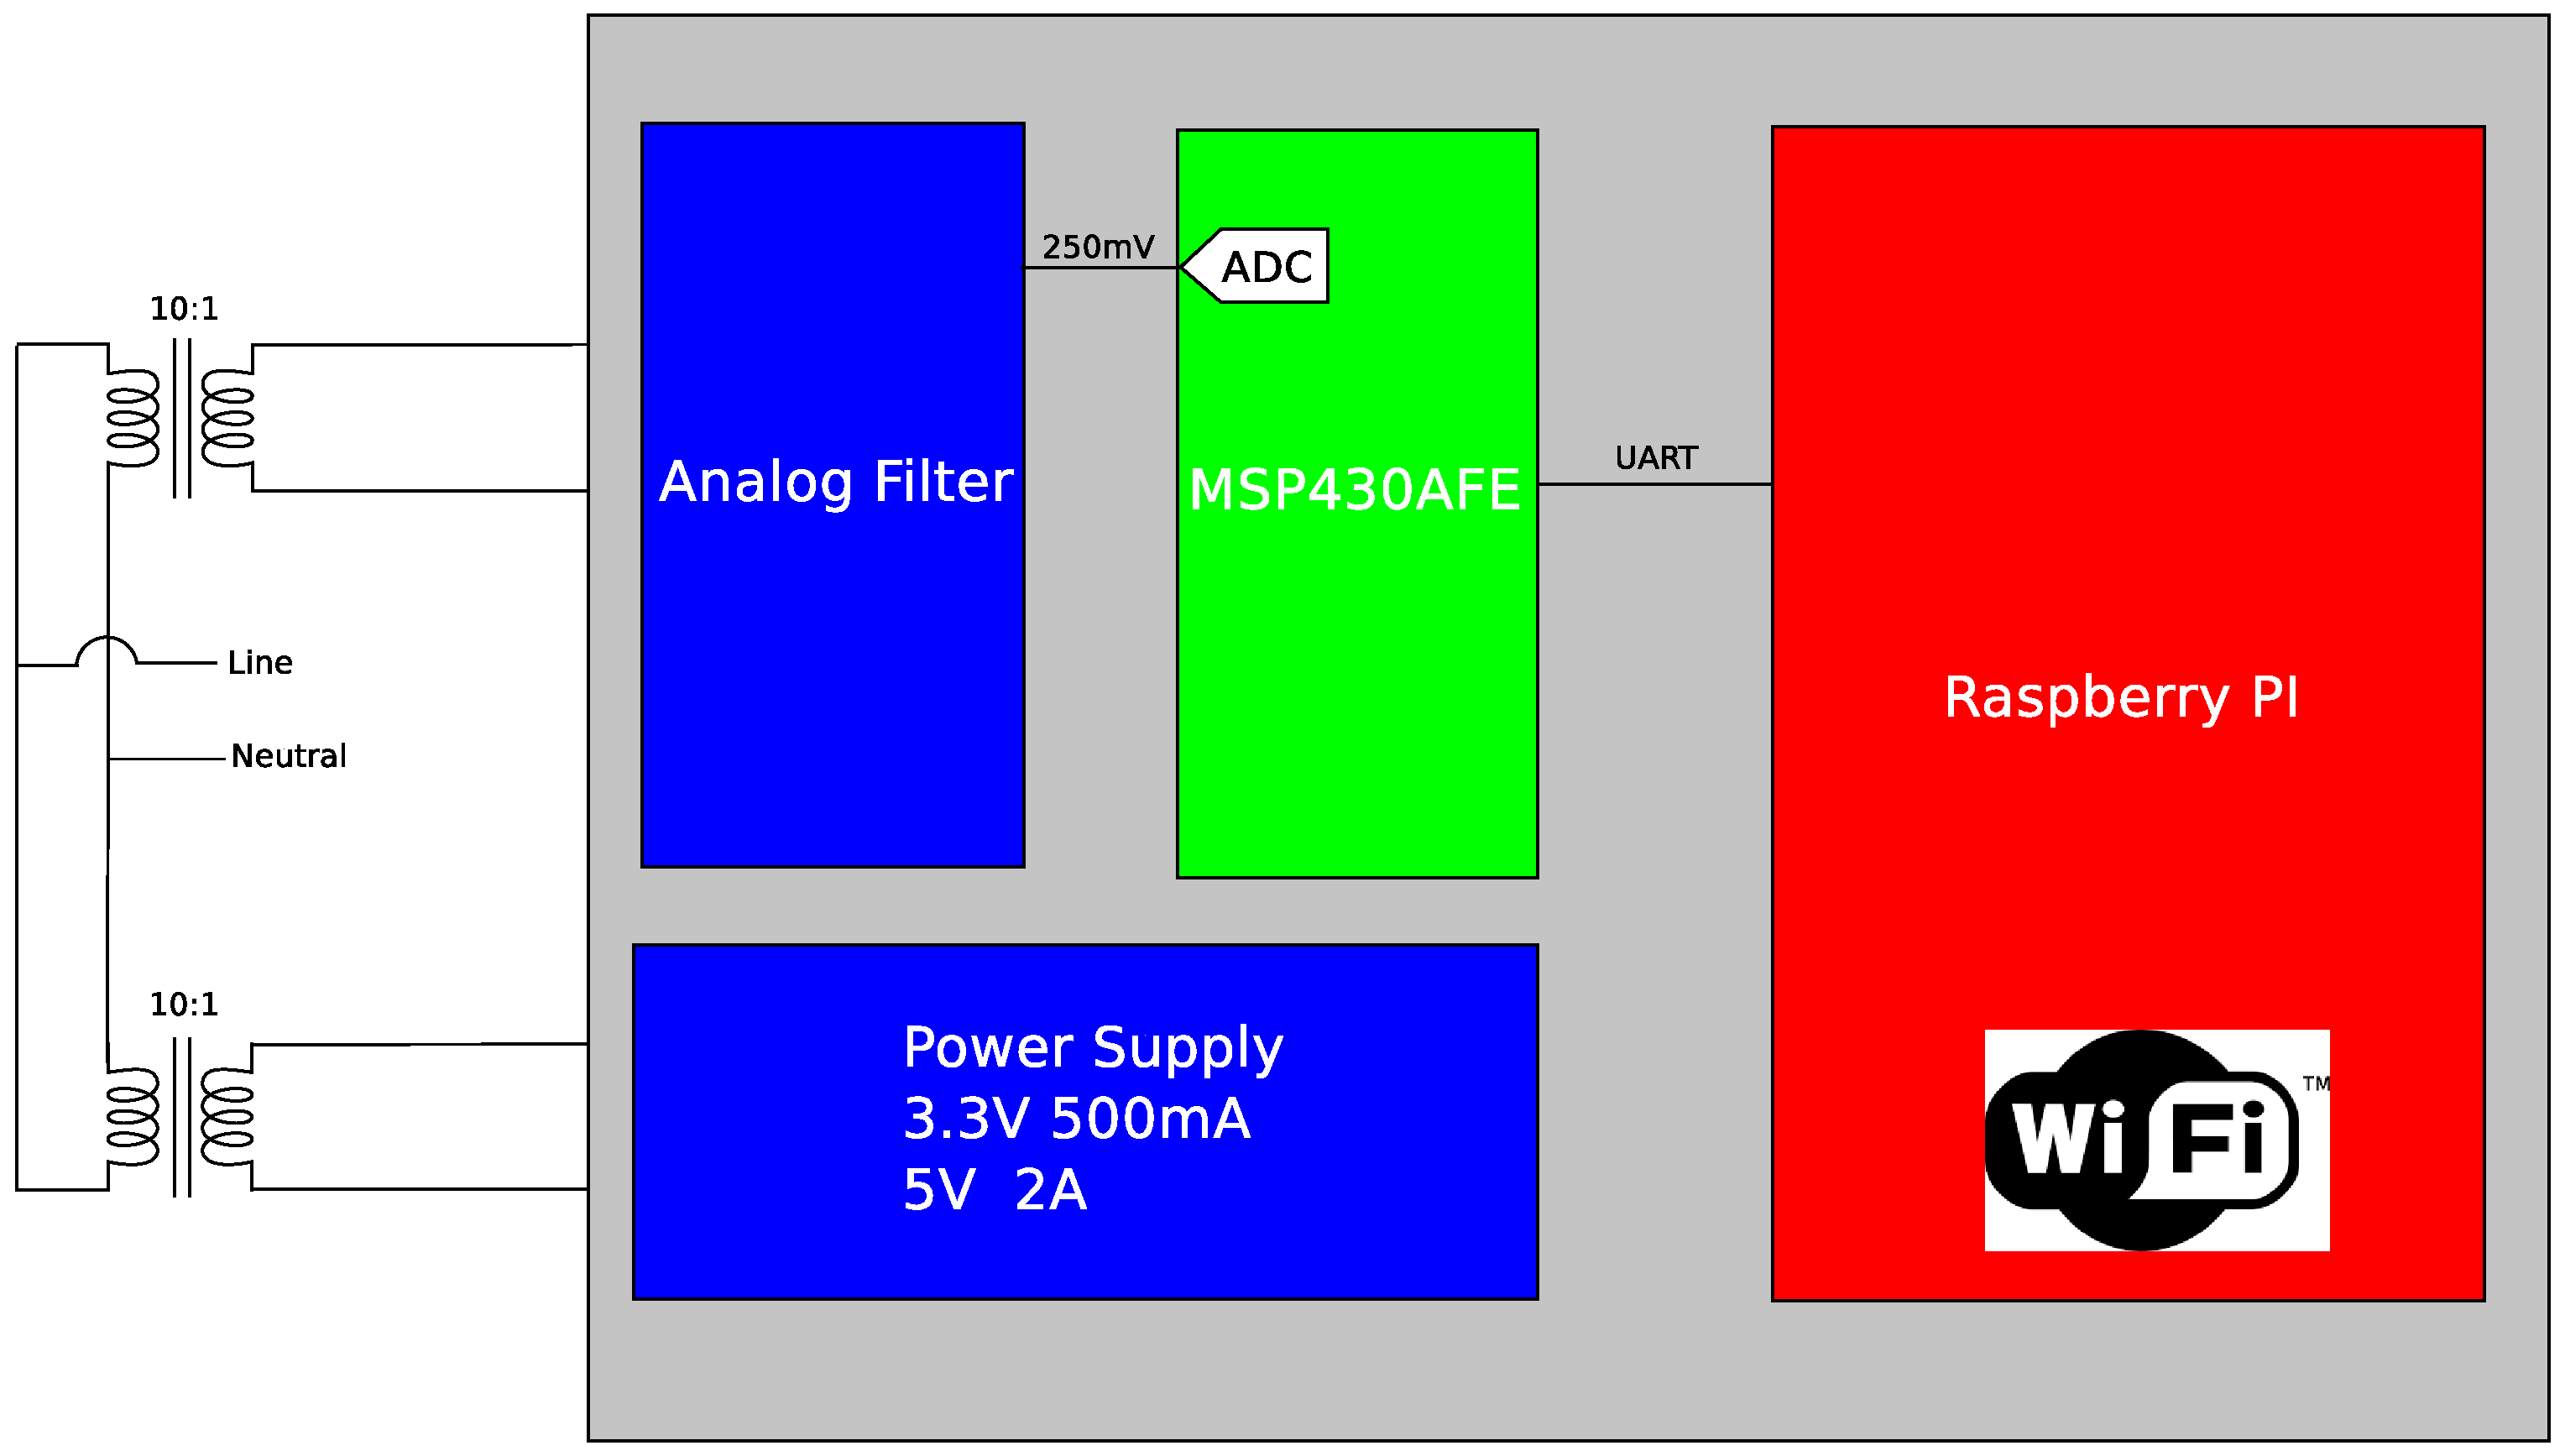
\includegraphics[width=0.7\textwidth]{img/OHM1Block.eps}
\caption{OHM1 Block Diagram}
\end{figure}

	At the heart of the device is the MSP430AFE integrated circuit by Texas Instruments \textregistered. This innovative device combines a 24bit $\Sigma\Delta$ analog to digital converter(ADC),
along with an MSP430 CPU core. MSP430 cpu core controls the hard real-time acquisition tasks, however with the peak of 8 MIPS, 512 bytes of RAM and no floating point unit, this device is not
capable to analyze the data it is gathering on its own. The soft real-time analysis is performed on a raspberry PI single board computer(SBC). Raspberry Pi is readily available SBC based on an 800Mhz
ARM11 SOC by broadcom. It features a high variety of digital peripherals, fast CPU with FPU and 512MB of memory. Furthermore this SBC is well supported by the Linux kernel and userland, 
with most drivers being open source and highly stable. The SBC reads and accumulates the ADC values generated by the MSP430 via a serial link. Once 4000 samples, or 1 second worth of data
have been gathered SBC performs rudimentary analysis and send interesting events, and overall statistics to the cloud via WIFI. Synchronization between devices is accomplished via disciplining the 
local clock with NTP.

\section{Acquisition Design.}
In order to measure the line voltage, it must first be scaled down to the ADC input range. This is performed in two stages. First a 10:1 transformer which isloates the circuit from the mains
, as well as steps down the $120V_{rms}$ to $12V_{rms}$. Next a passive network further scales the $12V_{rms}$ input to $200mV_{pp}$. Finally MSP430AFE digitizes the signal via a 24bit $\Sigma\Delta$
ADC. The 1bit ADC samples at 1Msps with the oversampling rate of 256 to achieve the 24bit resolution and 4kHz sampling rate. The state machine for the MSP430 CPU core is shown below.
\begin{figure}[h!]
\centering
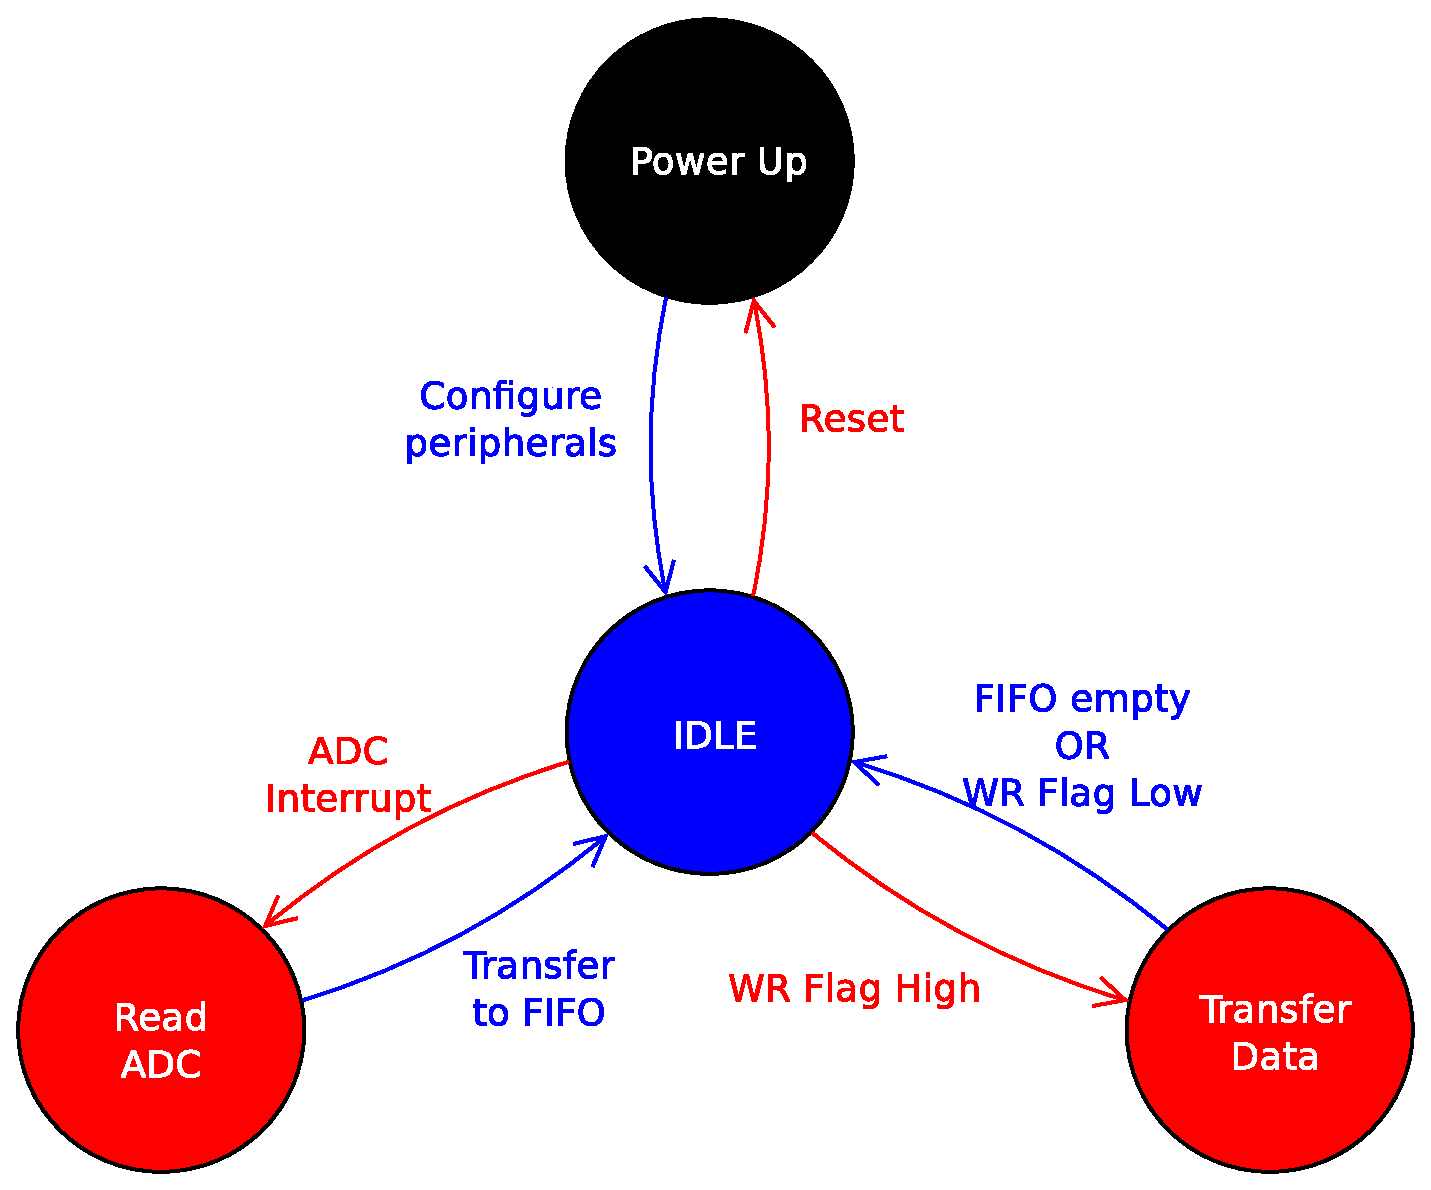
\includegraphics[width=0.5\textwidth]{img/MSP430StateMachine.eps}
\caption{MSP430 State Machine}
\end{figure}

	At startup MSP430 sets up the ADC, internal clocking and UART interfaces. Once the setup is finished it enters the IDLE state where the main CPU is in the low power mode. It remains in this mode
untill one of the three conditions are met:
\begin{enumerate}
\item \textbf{Reset line is pulled low.} In this case the CPU will reconfigure all of the peripherals, and enter the IDLE state once more.
\item \textbf{ADC interrupt fires.} This signifies that a new ADC sample is ready.
\item \textbf{WR Flag is pulled low.} This asserts that the Raspberry PI is ready to receive voltage samples.
\end{enumerate}
	
ADC is operating in the free-running mode, meaning, that the conversion timing is controlled via hardware. Once the conversion is complete a system interrupt notifies the CPU.
In order to remove the hard real-time constraint for the Raspberry PI, MSP430 CPU stores the ADC readings in an 85 sample FIFO. This FIFO, implemented as a circular buffer, 
allows the Raspberry PI to receive data at non-regular intervals. This is important since Raspberry PI is running a non real-time operating system. If the FIFO is full, the oldest sample
is dropped from FIFO. Unfortunately there is no mechanism to inform the Raspberry PI of an overflow in OHM1. This is remedied in the next iteration of the meter. See Chapter \ref{chap:further}
for more details on the future device revisions.

Communication between the Raspberry PI and the MSP430AFE is performed via UART with an addition of a WR line. When the WR line is pulled low, a level triggered interrupt notifies the MSP430 CPU
that the PI is ready for more data. The data is transfered via UART running at 230400bps.

\section{Data filtering and analysis}
	Raspberry PI is responsible for selecting events which deviate from the steady state condition. In our case steady state is a sinusoid with a set frequency and amplitude. Acquisition and processing
is performed in five steps:
\begin{enumerate}
\item Acquisition.
\item FFT/Peak fitting.
\item RMS calculation.
\item Event Filter.
\item Communication.
\end{enumerate}

	Acquisition step accumulates a 4000 sample window, and passes it on for processing. In order align the data during aggregation a millisecond timestamps is generated for each window.
Next the fundamental frequency of the waveform is computed. In order to do that a Fourier transform of the sample window is performed. Six points surrounding the largest FFT peak are selected,
and fitted  with a Gaussian in order to extract the true utility frequency.  

\begin{figure}[h!]
\centering
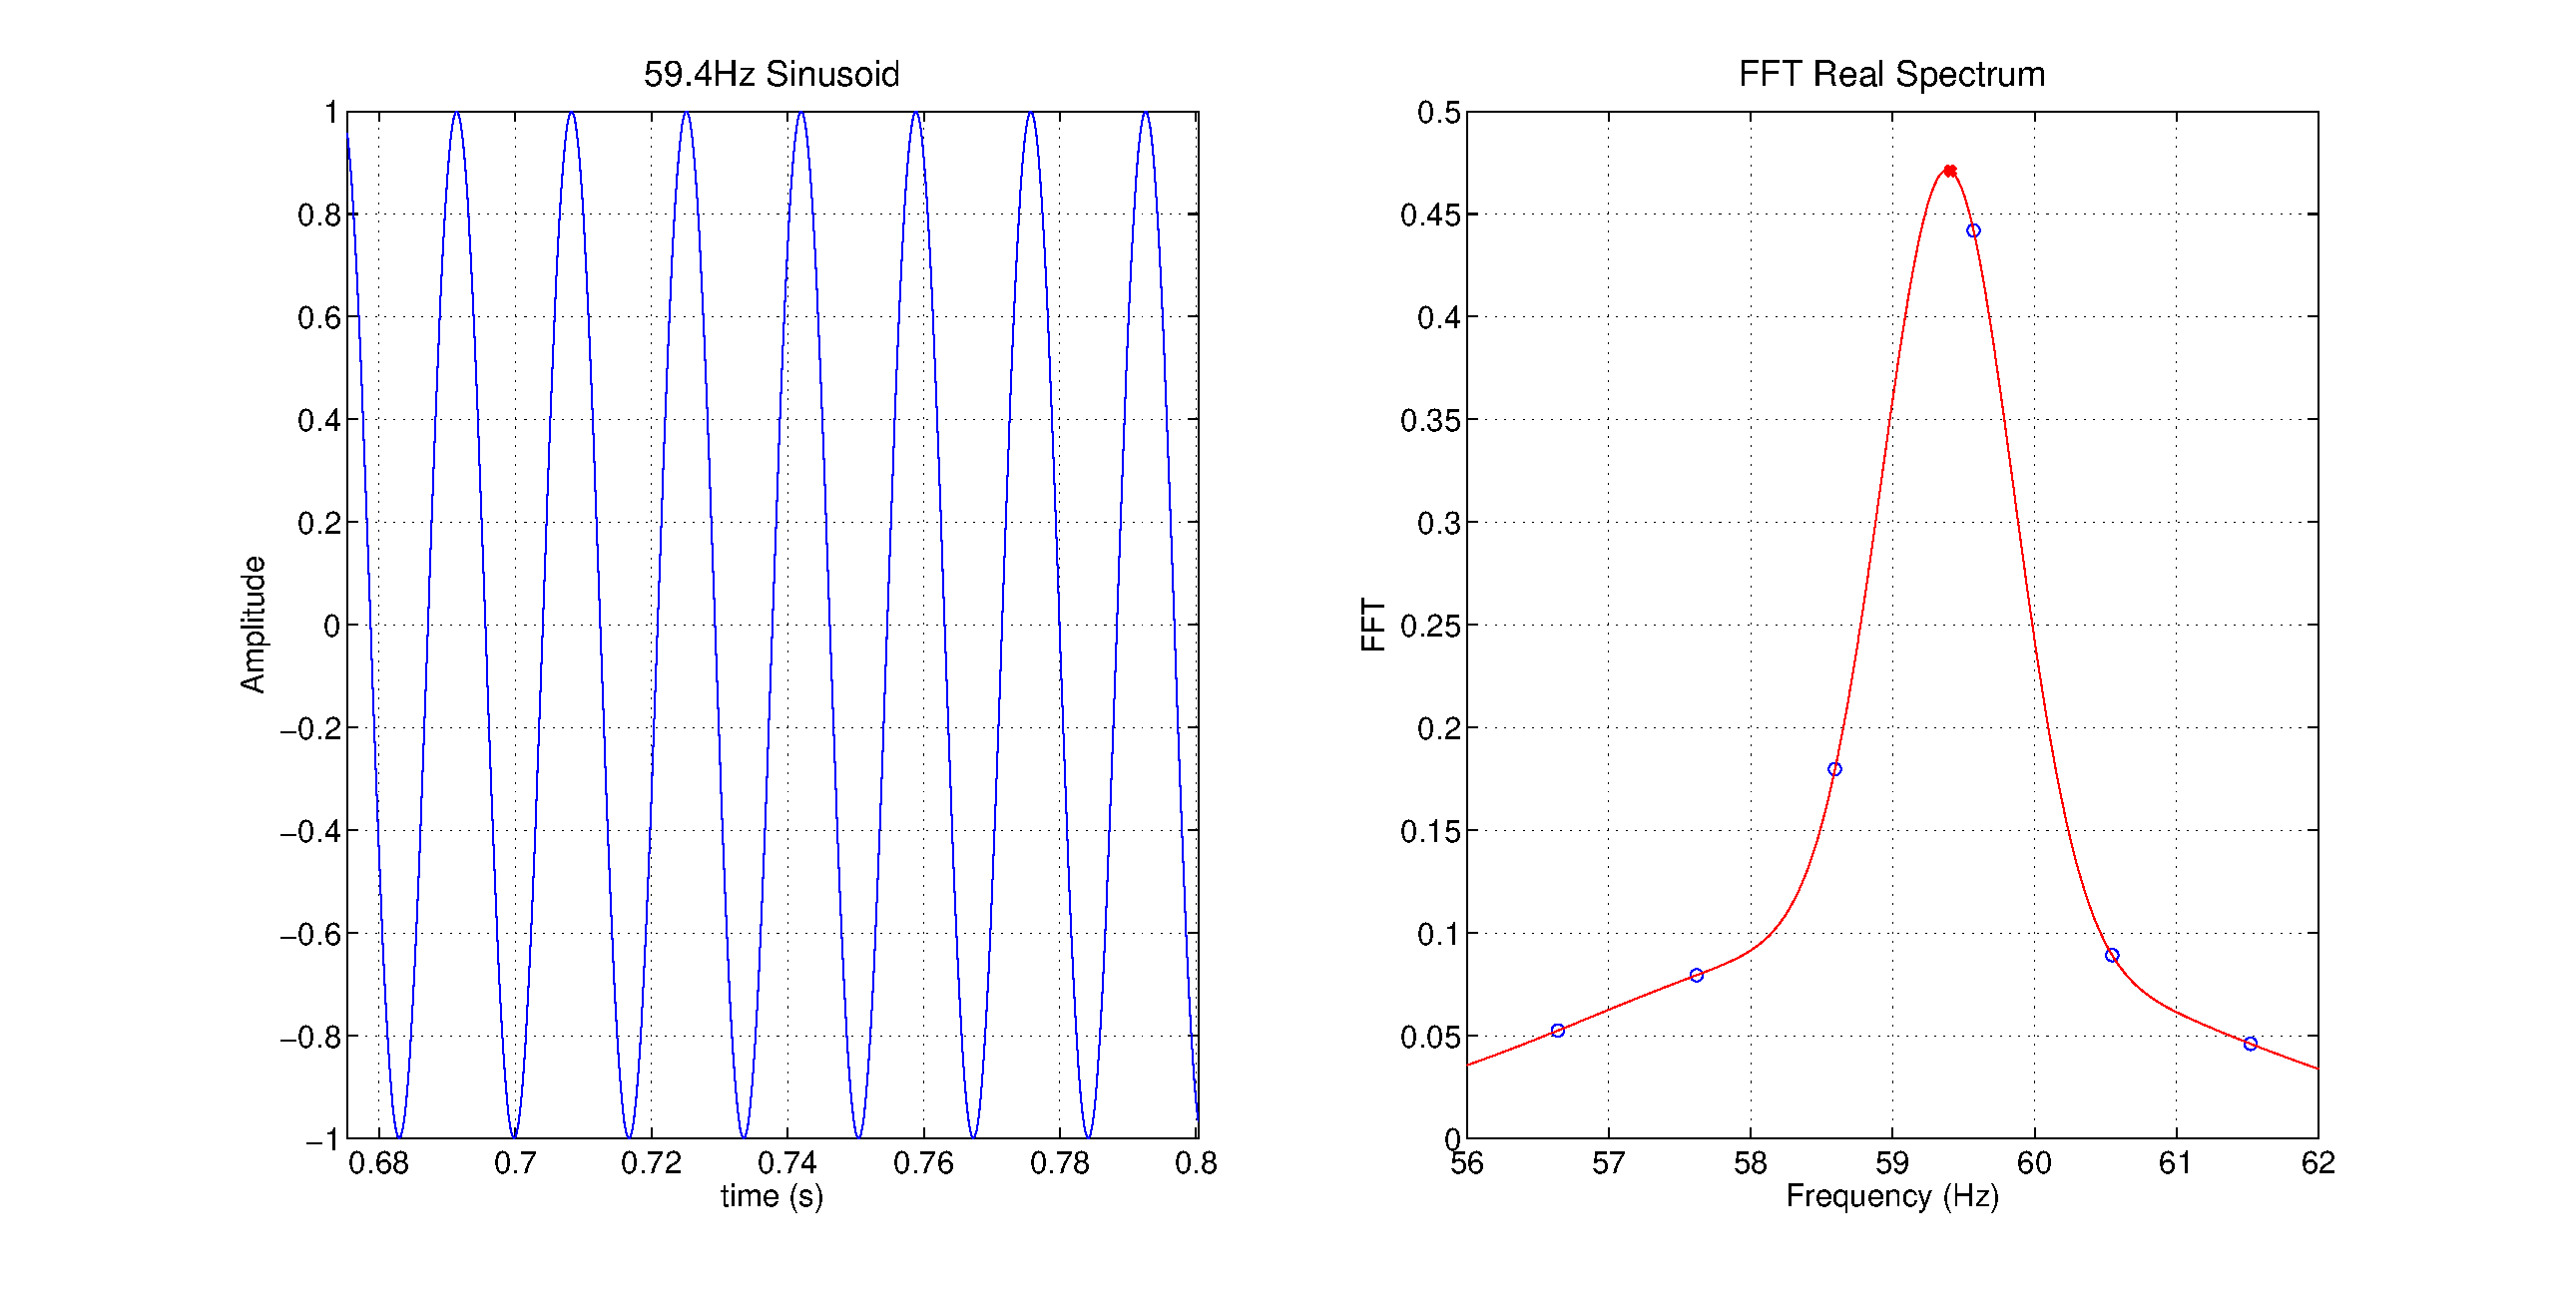
\includegraphics[width=\textwidth]{img/fftFit.eps}
\caption{Calculating the fundamental frequency using FFT and peak fitting.}
\textit{Left:} 59.3Hz sinusoid. \textit{Right:} Gaussian fit to the 6 point stradeling the peak.\\
Extracted maximum is 59.34Hz.
\end{figure}


Next Ohm1 calculates the RMS voltage. Only complete half-periods are included in this calculation, and the leading and trailing samples are pruned. The calculation is performed according to equation
\ref{eq:rms}

Every window recorded passes through the first three steps in OHM1 analysis system. However if the frequency and voltage are within tolerance, there is no reason to send it to the aggregation service.
In order to monitor the voltage and frequency trends however every 15th window is sent to the aggregation service regardless. If the utility frequency or rms voltage fall out of bounds the whole window is 
sent to the aggregation service as well. Filter task check the computed values against the tolerances and selects events to send to the cloud. We defined our tolerances to be:
\begin{itemize}
\item $\pm 0.5Hz$ deviation from the $60Hz$ norm.
\item $\pm 7V_{rms}$ deviation from the $120V_{rms}$ norm.
\end{itemize}

Finally a window is ready to be sent to the aggregation service. Raspberry PI maintains a connection to the service via a WIFI dongle. If a window is selected to be sent to the aggregation, it is
serialized into JSON, along with the appropriate metadata, and sent over a websocket connection.

\section{Aggregation Infrastructure}
Open Power Quality aggregation software, titled OPQHub, is responsible for communicating with the OHM1 devices, and serving user side content. It is written in Java using the Play framework. 
\begin{figure}[h!]
\label{fig:opqhub}
\centering
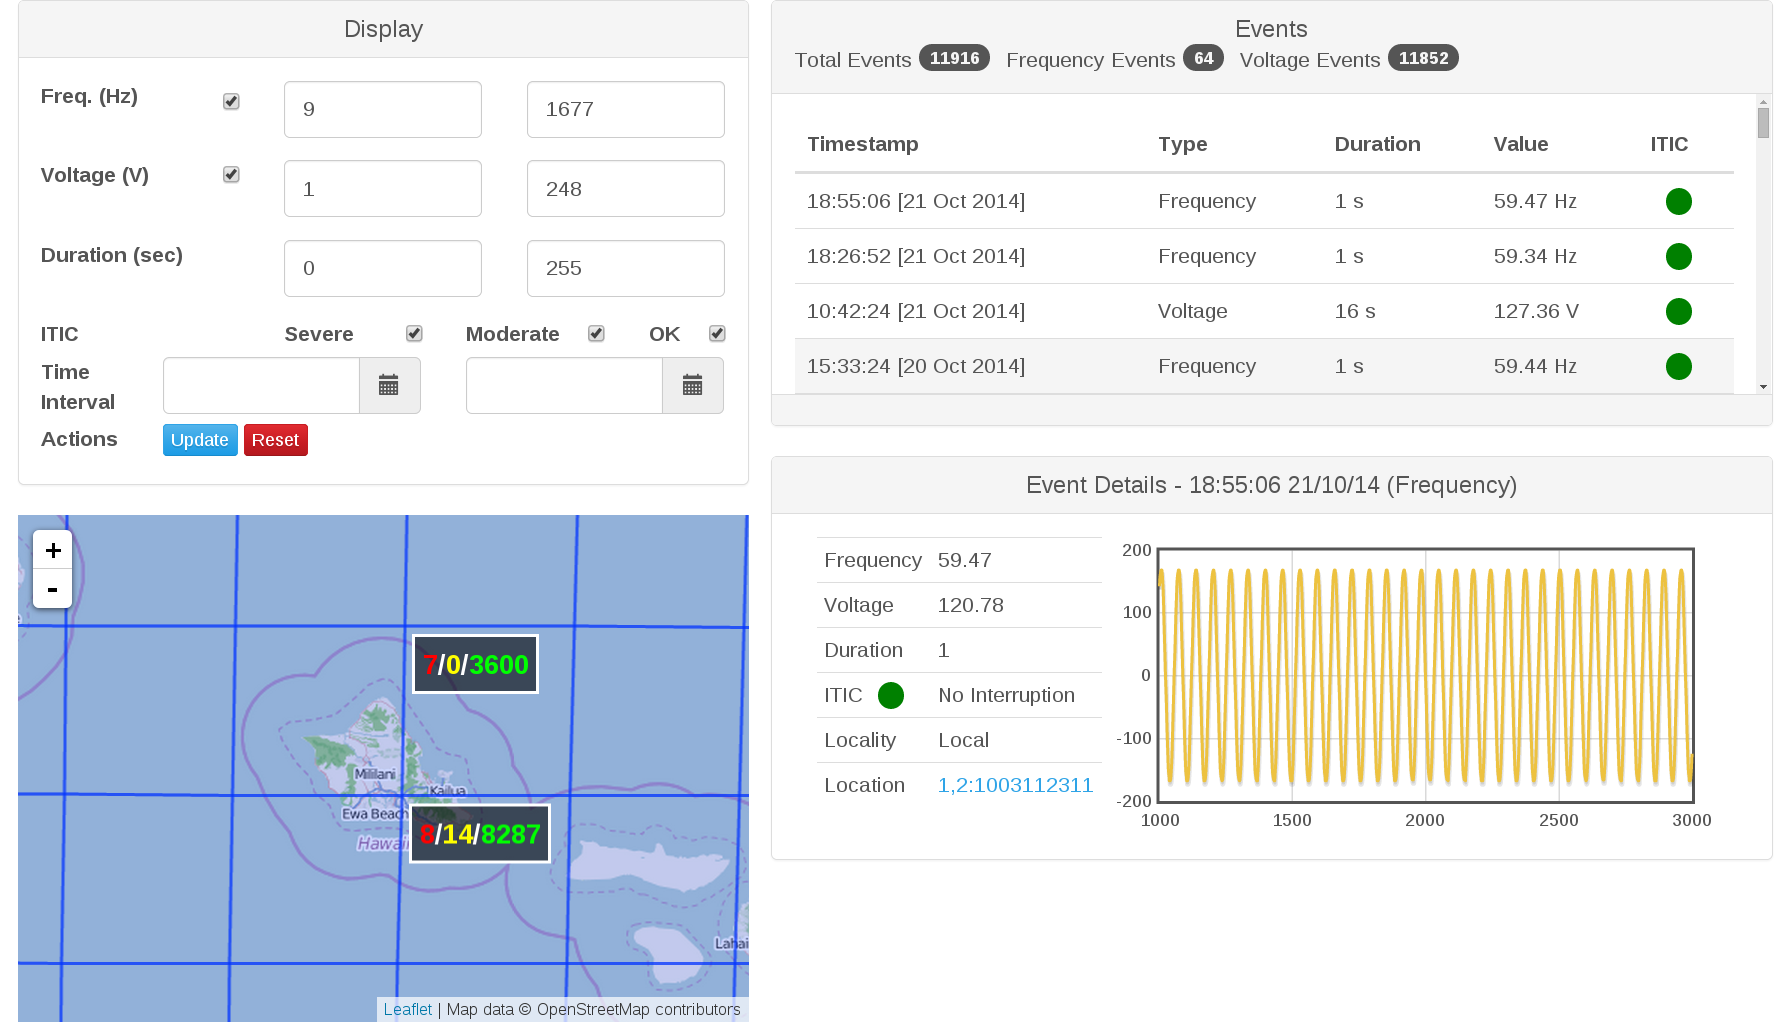
\includegraphics[width=0.8\textwidth]{img/opqhub.png}
\caption{OPQHub public interface.}
\end{figure}

OPQHub provides a rich visualization suit as shown in Figure \ref{fig:opqhub}, along with a data querying API for developers. Unfortunately description of the internal function
of such a feature rich, scalable architecture is beyond the scope of this paper. A white paper on this topic has been previously published by OPQ. Cite anthony!

\chapter{Results}

In this chapter we discuss the preliminary results of  OHM1 deployment. First we attempt to correlate the voltage trends to the output of a PV installation. Next we take a look at the 
waveform of an event recorder on two geographical separated devices.

\section{Grid Voltage and Grid Tied Photovoltaic Installations}
Top graph in figure \ref{fig:samehouse} shows the rms voltage recorded from August 1 to August 8 for a single device in a residential home. The bottom plot shows the power produced by 
a grid tied PV installation, located on the roof of the same house.

\begin{figure}[h!]
\centering
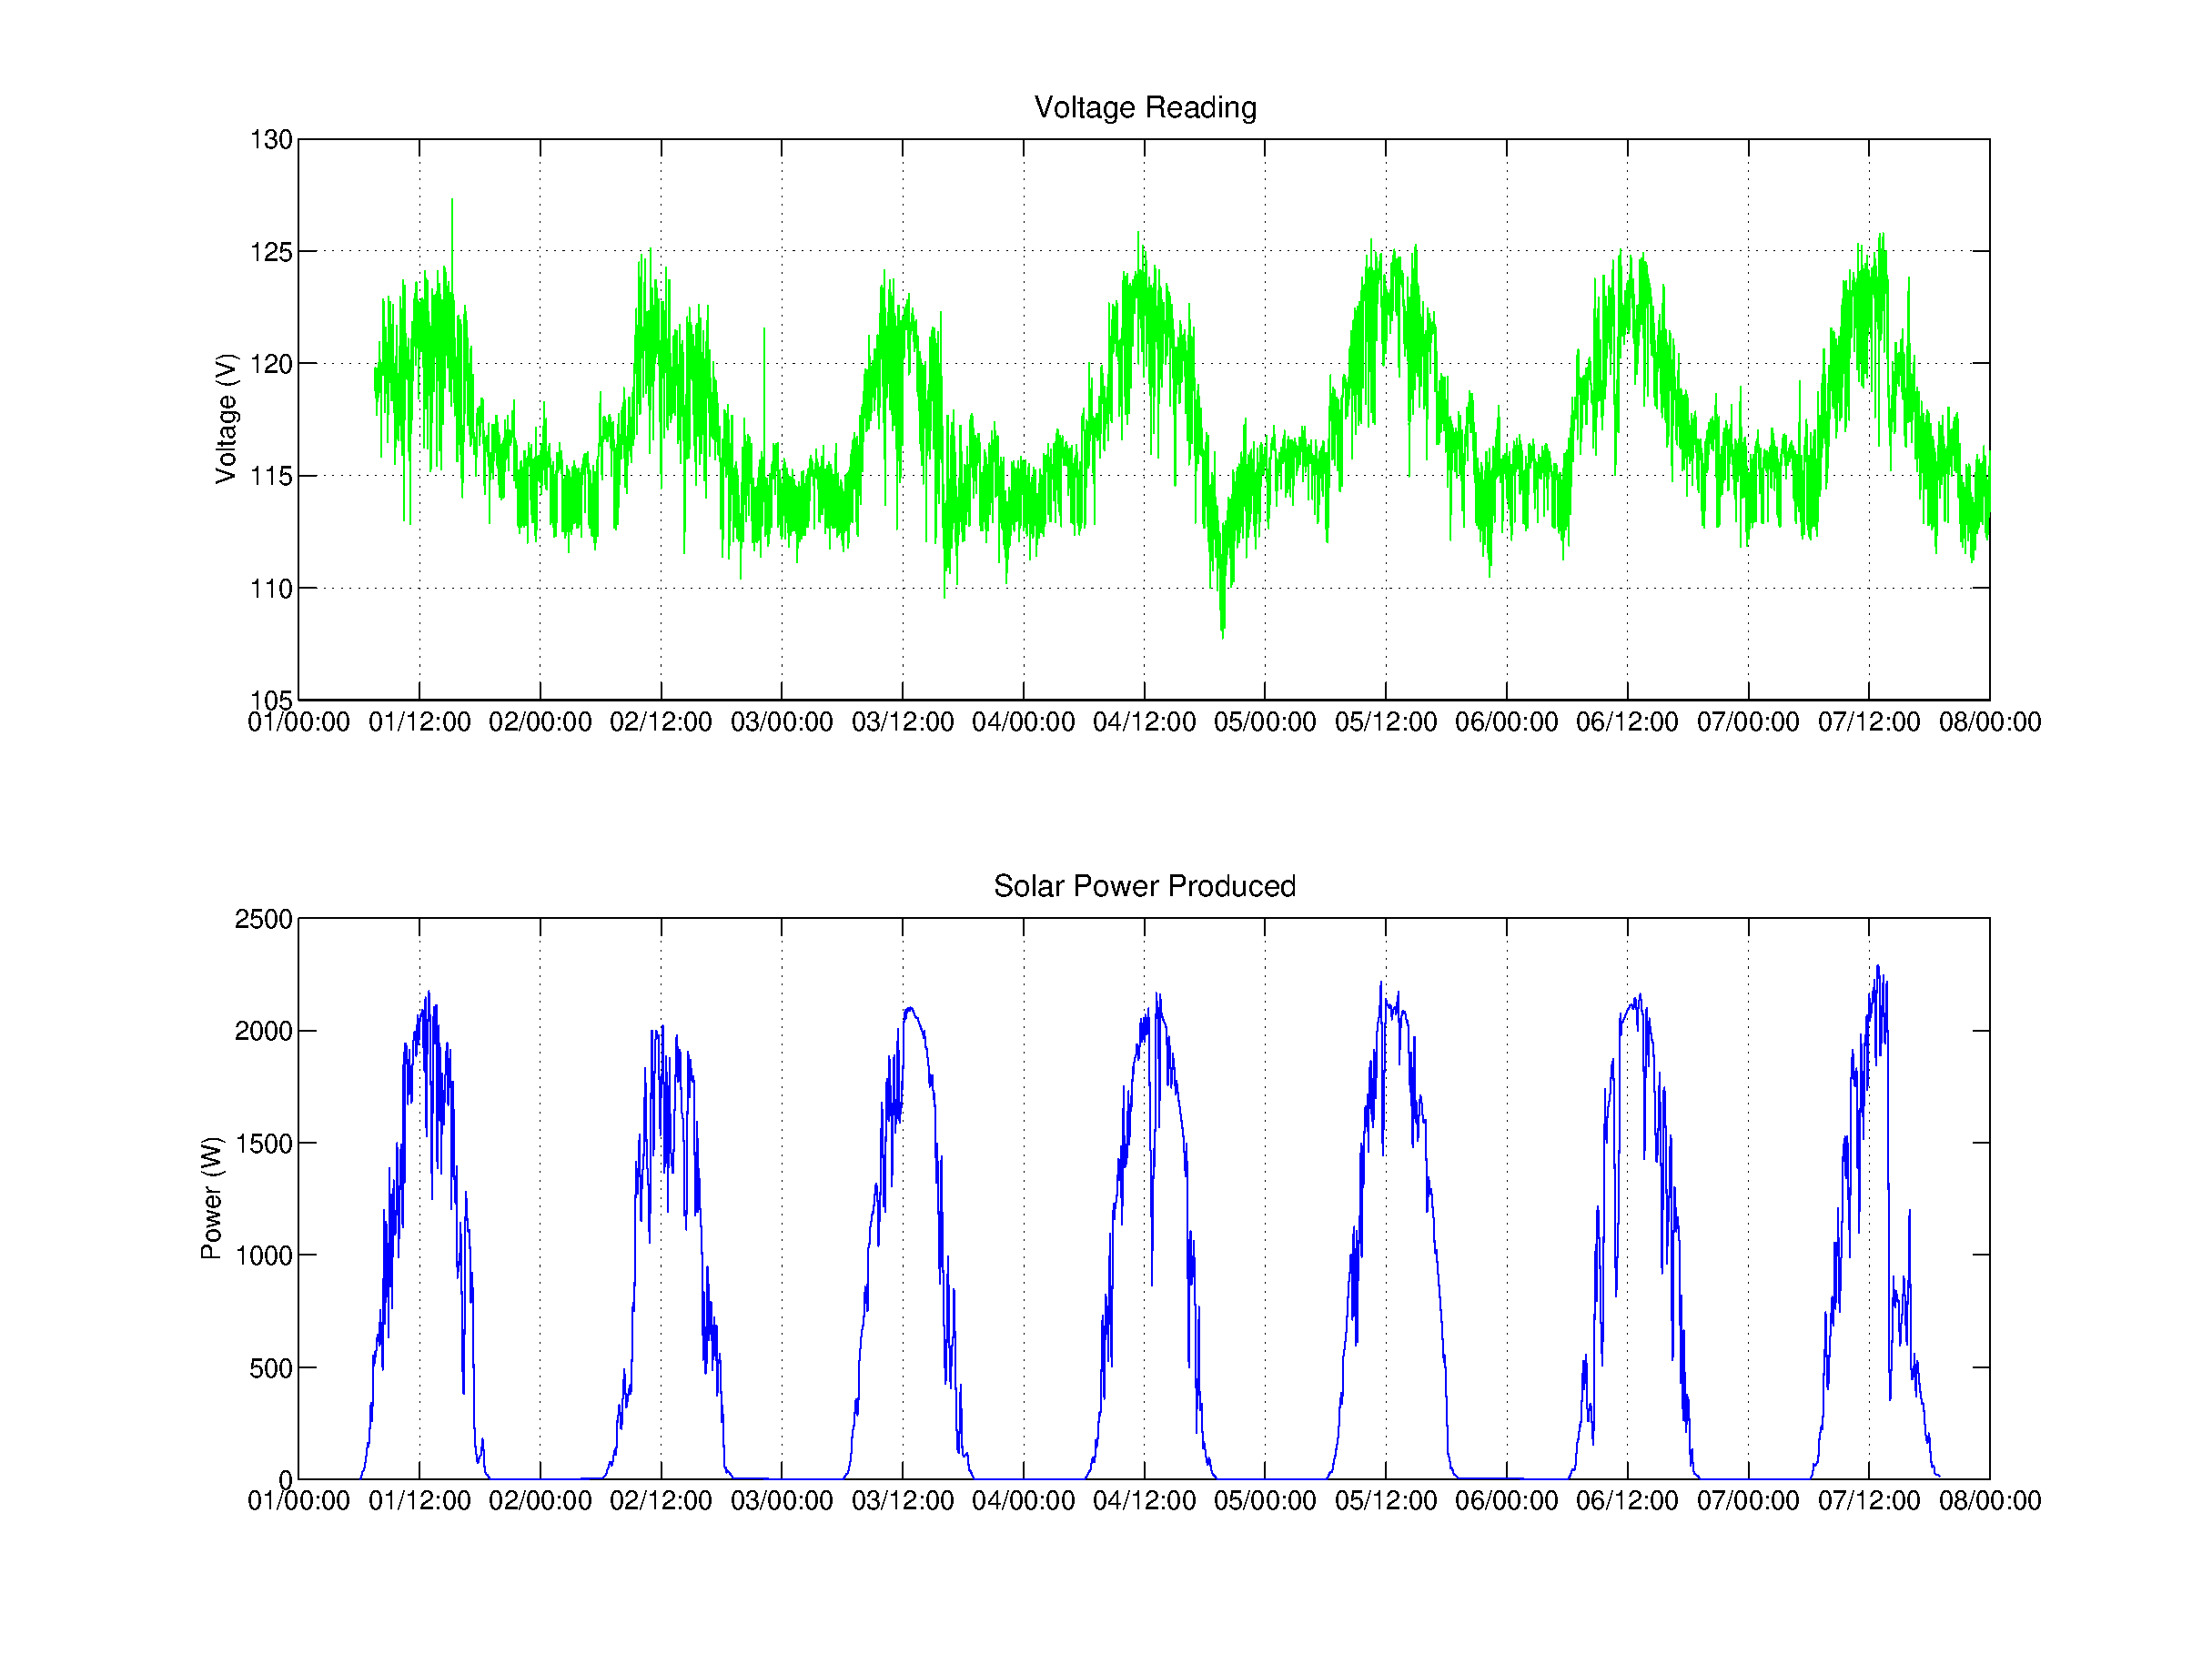
\includegraphics[width=\textwidth]{img/solarCorelationSameHouse.eps}
\caption{Grid voltage and solar power produced. Device and PV located in the same house.}
\label{fig:samehouse}
\end{figure}

The correlations between the power produced and the voltage are clearly shown in figure  \ref{fig:samehouse}. Some of the more fine-scale correlations are also visible. 
For example large drop in PV output on August 4 13:00pm is correlated to a drop in the utility voltage. This leads us to believe that solar panels contribute to the
variation of the line voltage of the house they are supplying. This begs the question: how do photovoltaics influence the grid voltage as a whole?

\begin{figure}[h!]
\centering
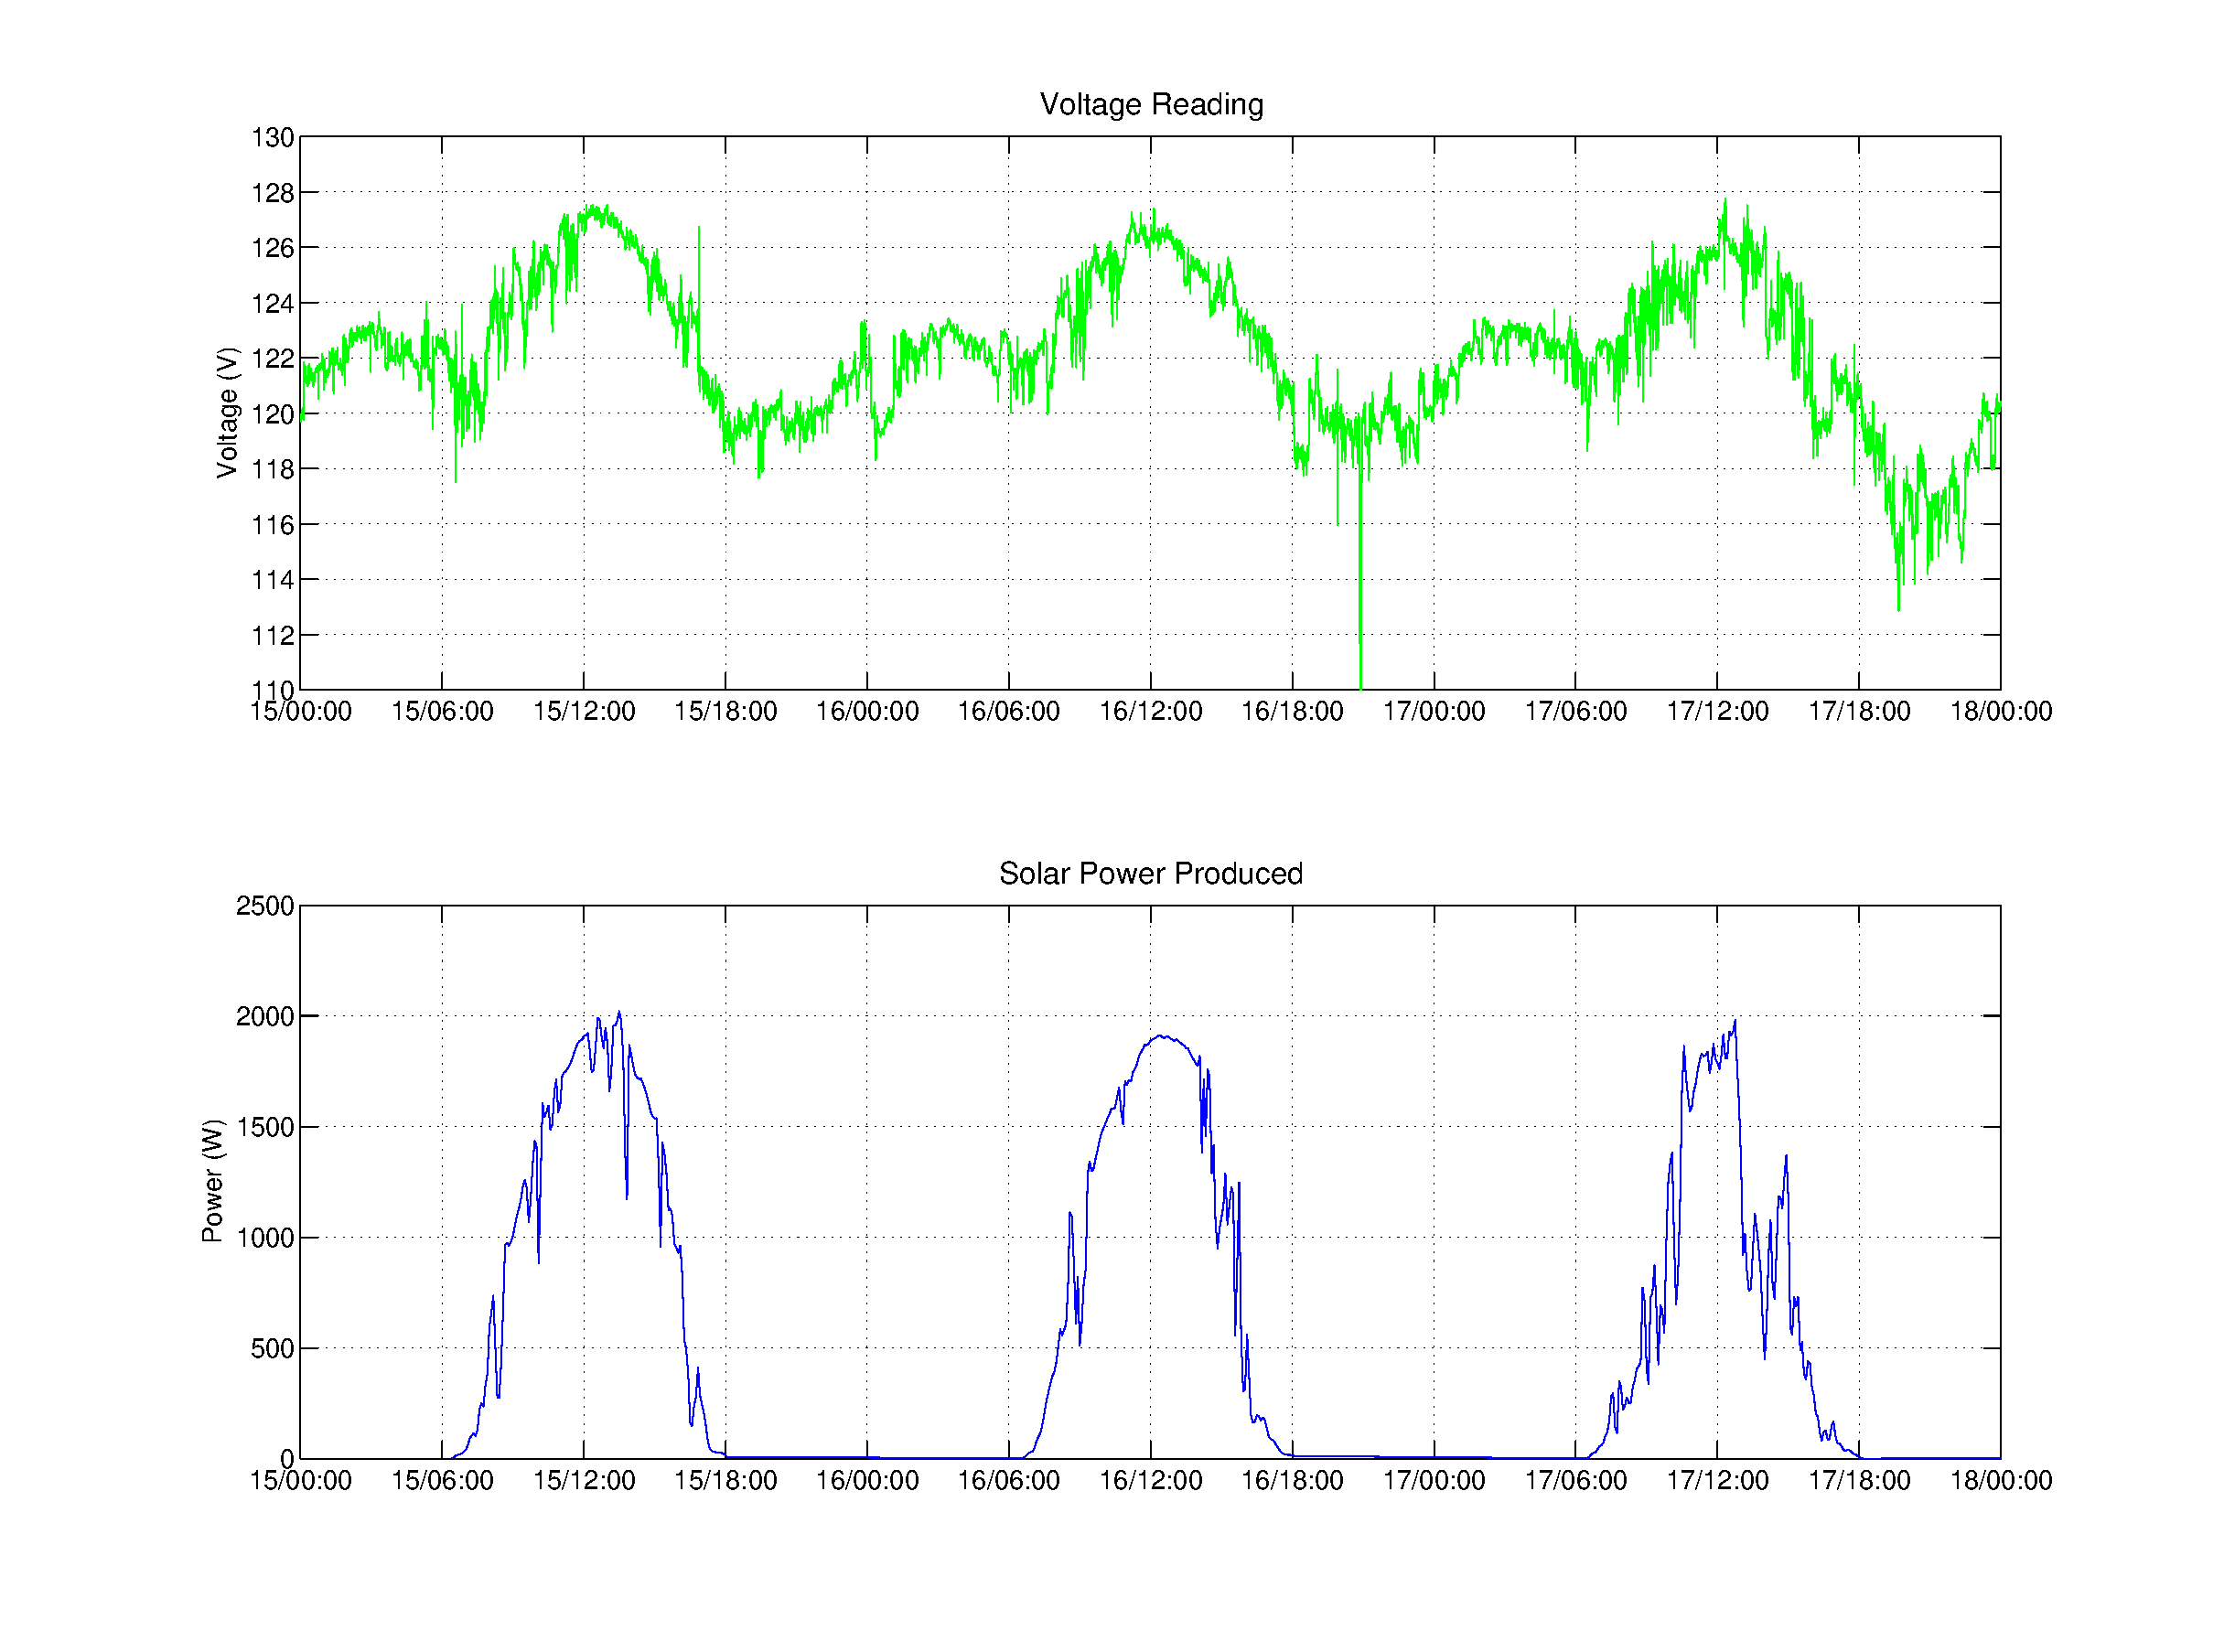
\includegraphics[width=\textwidth]{img/SunnyWeather.eps}
\caption{Grid voltage and solar power produced. Device and PV located are separated by ~20 miles.}
\label{fig:diffhouse}
\end{figure} 

Figure 3.2 shows the same to graphs as figure 3.1 for October 15 to October 18. This time however OHM1 device and the Photovoltaics unit are separated by 20 miles. The house
containing the device did not have a grid tied PV system. Correlations are present nonetheless, line voltage measured by the device is proportional to the power generated by the PV installation.
A possible explanation for this effect is that PV installations affect the line voltage across the whole grid. Oct 15-17 were clear days with minimal cloud cover, which implied that PV
installations were generating power across the island, perhaps affecting the grid voltage while doing so. One way to answer this question is examine the line voltage trend while the PV installations
across the island are idle. 

On the days of October 17 through October 19 hurricane ANA passed within 100 miles of the island of Oahu. Its passing brought heavy clouds which enveloped the entire island. Clouds began to form 
late afternoon Friday, October 18, as demonstrated by the power generation drop in figure 3.2 along with the line voltage drop recorded by the device. Voltage and Power reading for
October 18 through October 20 are shown in figure 3.3.

\begin{figure}[h!]
\centering
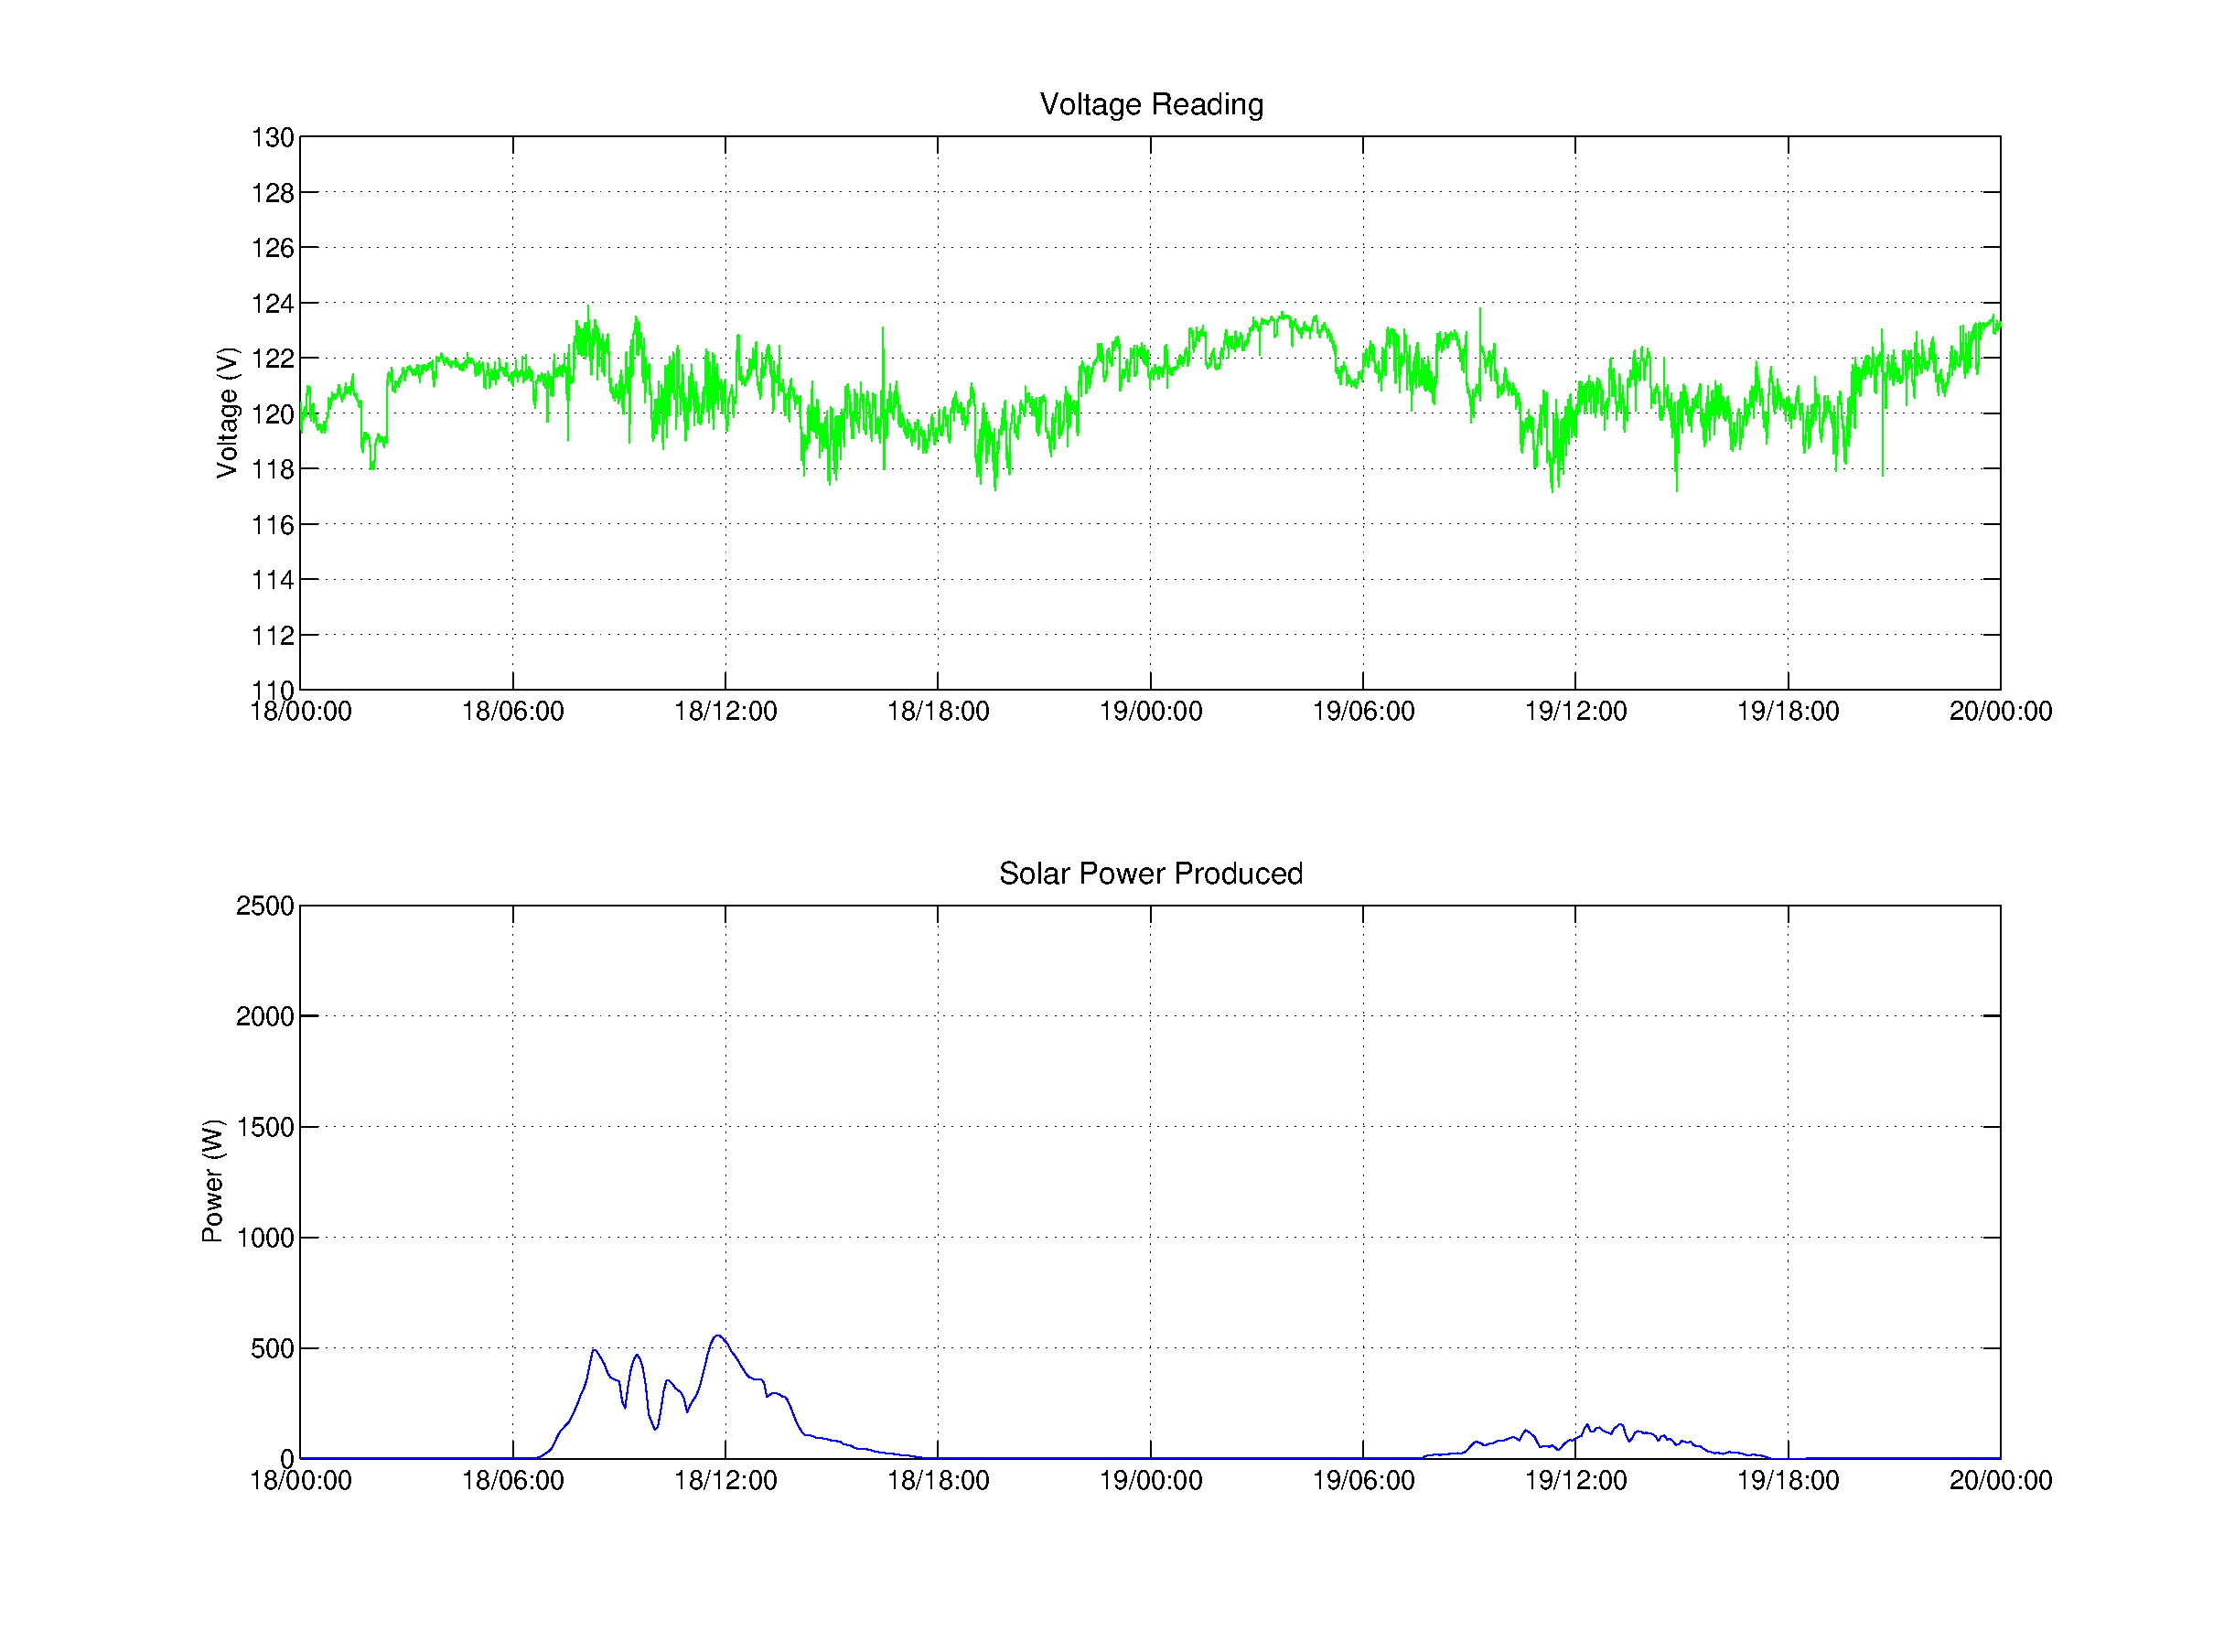
\includegraphics[width=\textwidth]{img/Stormy.eps}
\caption{Grid voltage and solar power produced during hurricane Ana. Device and PV located are separated by ~20 miles.}
\label{fig:storm}
\end{figure} 

During peak hours, the PV installation from  Figure 3.2 was generating 2kW of power, yet during the storm on October 18 and 19 it was generating 550W and 100W respectively. Furthermore
the line voltage did not exhibit the same variations we saw in figure 3.1 and figure 3.2. While more research is required, data we collected over the last several months shows that the
high penetration of PV installations on Oahu is affecting the grid voltage. The extent of this effect remains to be explored.

\section{Grid Wide Events}

As described in Section 2.3, our system is able record both long term trends, and short term transients. Unfortunately only several of such transients have been confirmed to be grid wide.
The best example of such an event is shown in figure 3.4.

\begin{figure}[h!]
\centering
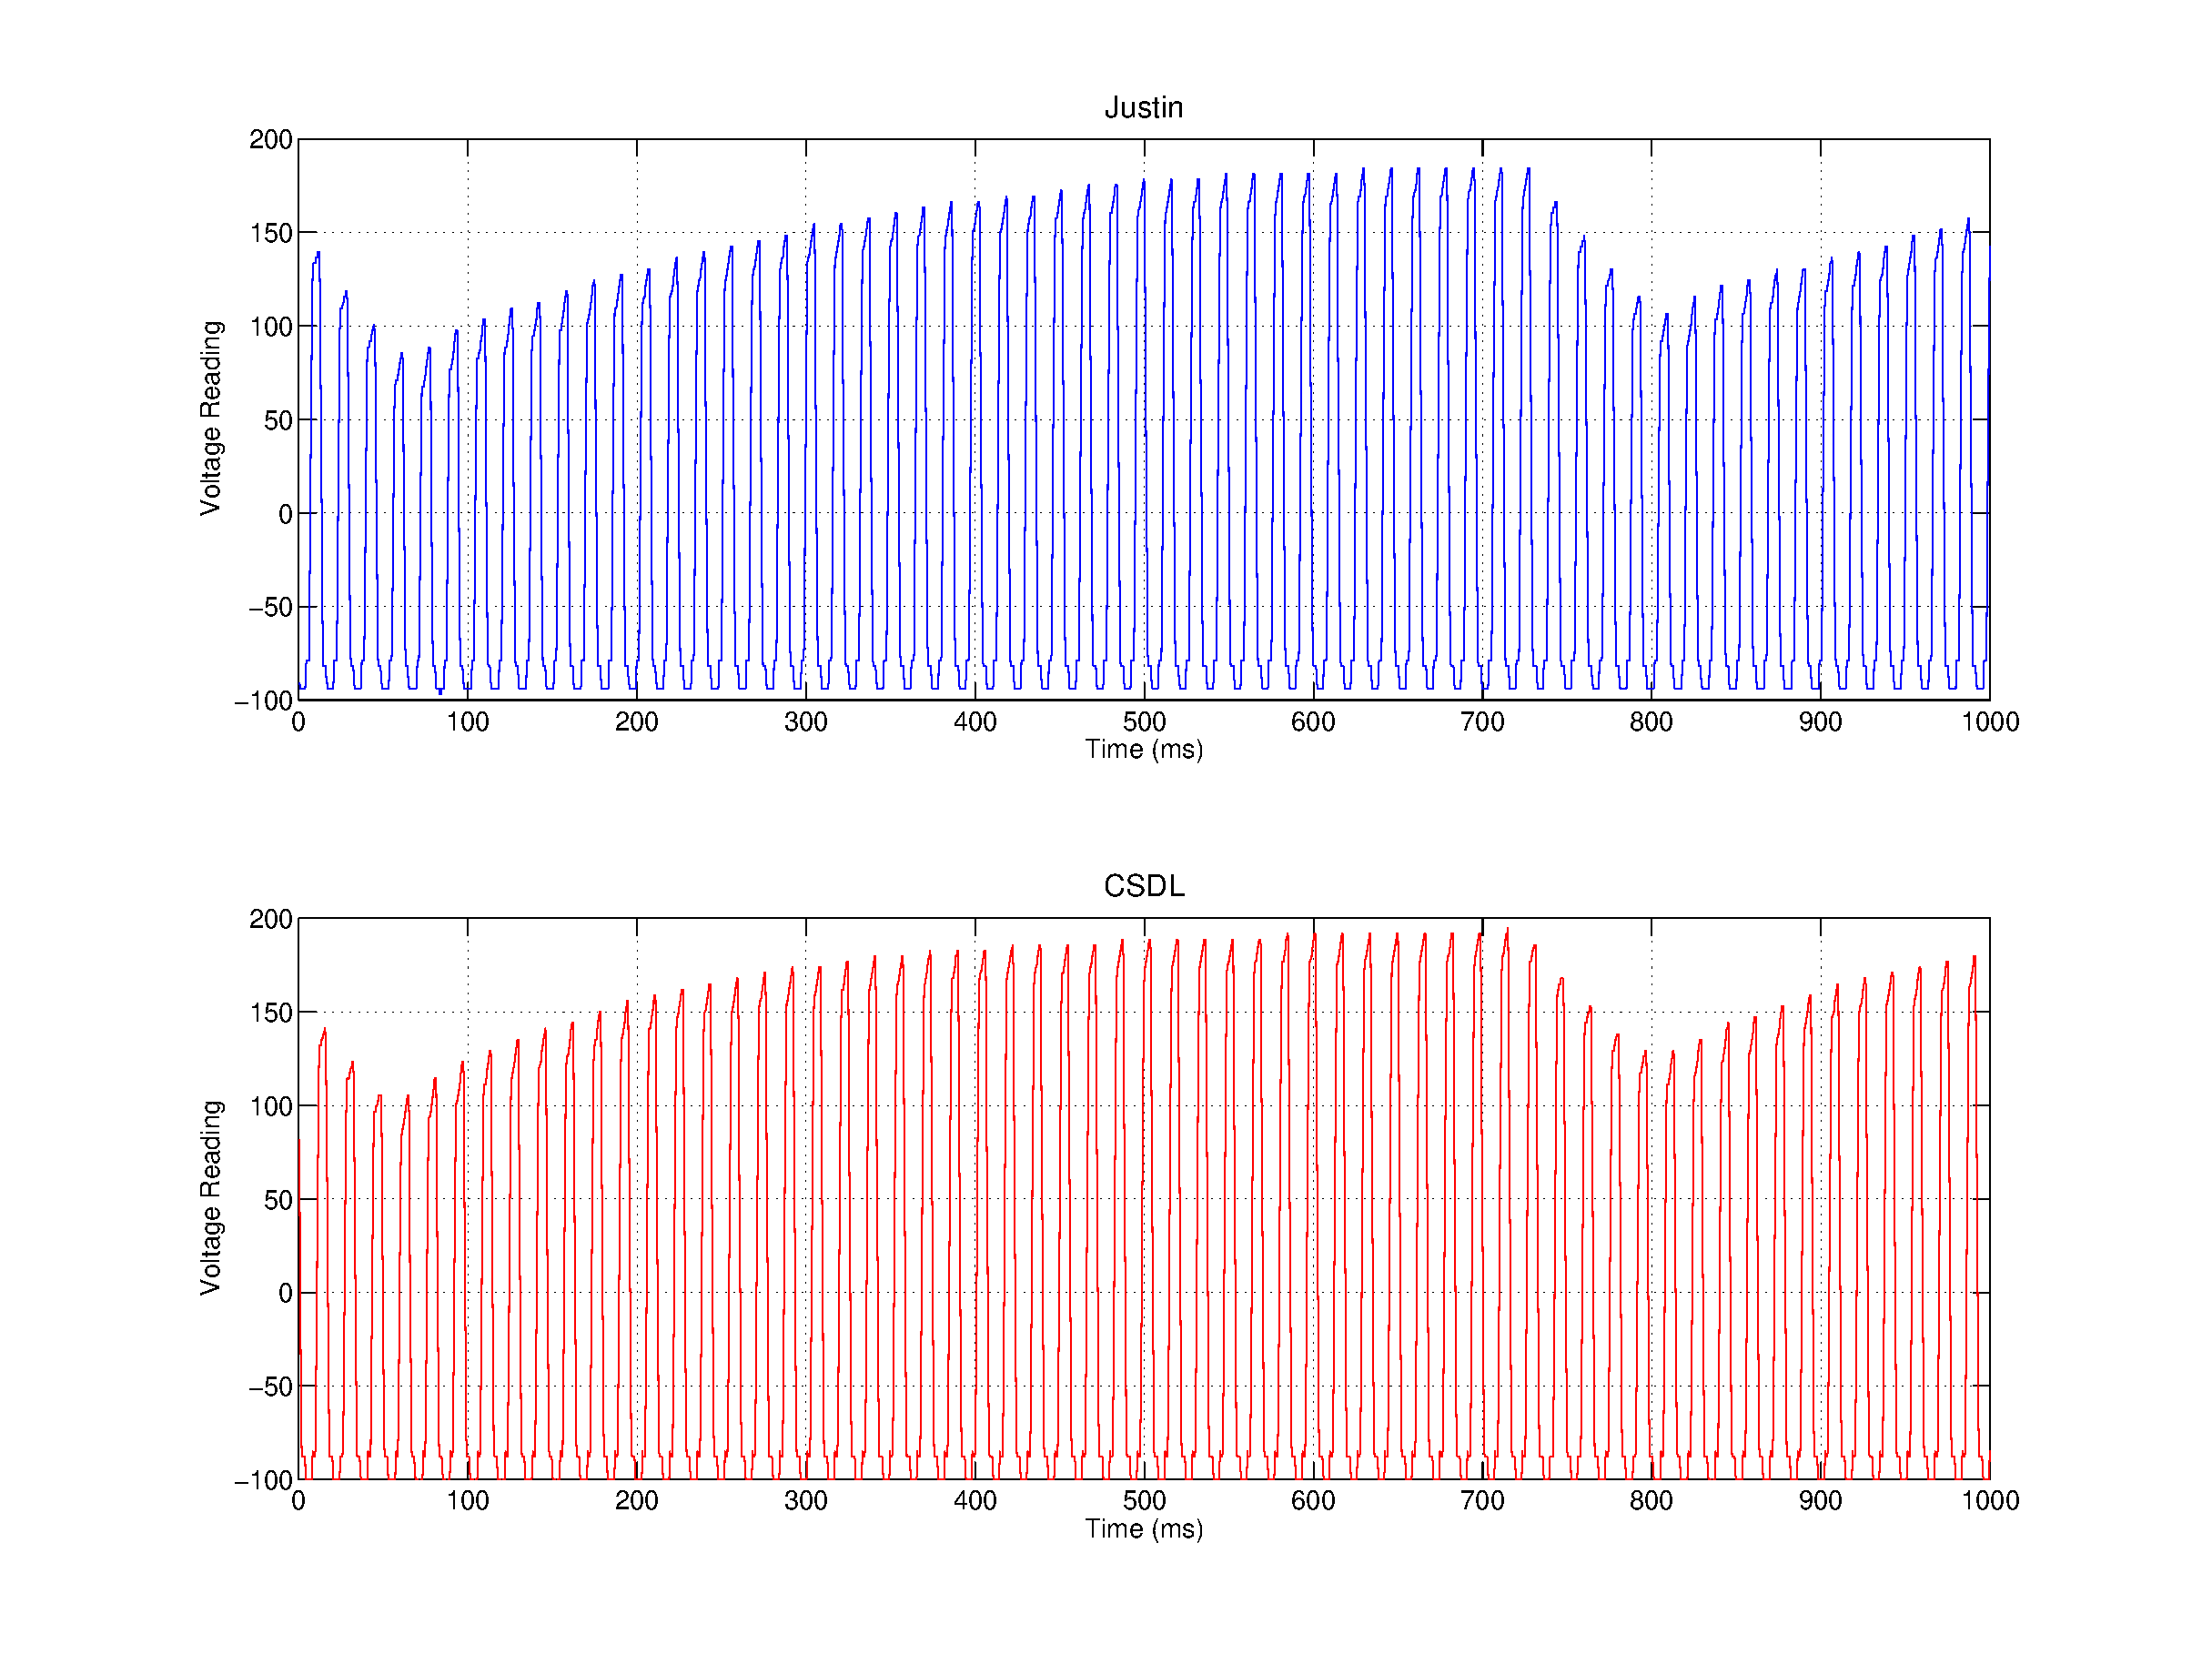
\includegraphics[width=\textwidth]{img/gridwide.eps}
\caption{Grid-wide event recorded by two devices on 13:46 on Sept 30. Devices are 10 miles apart.}
\label{fig:grid}
\end{figure} 

An event above is two voltage sags lasting 6 cycles, separated by ~700ms. It was seen by two devices, one located at University of Hawaii at Manoa, and the other 10 miles away in a high rise
apartment building. The timestamp between two waveforms differed by 18ms, or approximately one grid cycle. While the cause of this particular disruption will likely remain unknown, events 
such as this prove both the feasibility and the need for deployment of a power quality monitoring system such as OHM1 and OPQHub.

\chapter{Further Study}\label{chap:further}
	
\chapter{Conclusions}
